\documentclass[12pt,a4paper]{article}
\usepackage[utf8]{inputenc}
\usepackage{graphicx}
\usepackage{amsmath}
\usepackage{amssymb}
\usepackage{float}
\usepackage{caption}
\usepackage{subcaption}
\usepackage{hyperref}
\usepackage{listings}
\usepackage{xcolor}

% Set up code formatting
\lstset{
    basicstyle=\ttfamily\footnotesize,
    numbers=left,
    numberstyle=\tiny\color{gray},
    stepnumber=1,
    numbersep=10pt,
    backgroundcolor=\color{lightgray!10},
    showspaces=false,
    showstringspaces=false,
    showtabs=false,
    frame=single,
    rulecolor=\color{black},
    tabsize=4,
    captionpos=b,
    breaklines=true,
    breakatwhitespace=false,
    keywordstyle=\color{blue},
    commentstyle=\color{green!50!black},
    stringstyle=\color{orange},
}

\title{Communications Project: Frequency Division Multiplexing (FDM) using SSB Modulation}
\author{}
\date{Fall 2024}

\begin{document}

\maketitle
\begin{center}
    \vspace{1cm}
    \textbf{Presented to:} \\
    Michael Melek
    \vspace{1cm}
\end{center}

\begin{center}
    \vspace{1cm}
    \textbf{Presented by:} \\
\begin{tabular}{|c|c|}
    \hline
    \textbf{Name} & \textbf{ID} \\
    \hline
    Moamen Moahmmed & 9220886 \\
    \hline
    Mina Hany & 9220895 \\
    \hline
\end{tabular}
\end{center}

\newpage

\tableofcontents
\newpage

\section{Introduction}

This project explores the modulation of three speech signals using single sideband (SSB) modulation within a frequency-division multiplexing (FDM) system. The goal is to implement signal processing techniques such as low-pass filtering, modulation, and demodulation, ensuring high-quality transmission and recovery of signals.

\subsection{Objectives}
\begin{itemize}
    \item Record and process three voice signals.
    \item Filter the signals using a low-pass filter.
    \item Modulate the filtered signals using SSB modulation.
    \item Multiplex the modulated signals using FDM.
    \item Demodulate the multiplexed signal to recover the original signals.
\end{itemize}

\newpage

\section{Voice Signal Recording and Preprocessing}

\subsection{Recording Voice Signals}
The chosen sampling frequency is \texttt{44100 Hz}. This complies with the Nyquist theorem, which states that the sampling frequency must be at least twice the highest frequency component in the signal to avoid aliasing. Human speech primarily occupies the frequency range of 300 Hz to 3.4 kHz. By selecting a sampling rate of 44.1 kHz, the signal is accurately captured with no significant loss of high-frequency details. Furthermore, this sampling frequency ensures sufficient bandwidth to prevent distortion and aliasing during the modulation process, particularly as the signal's frequency content is shifted to higher frequencies during single-sideband (SSB) modulation. This choice supports the accurate transmission and recovery of the signals in the Frequency Division Multiplexing (FDM) system.

\subsection{Saving Recorded Signals}
The signals were saved as \texttt{input1.wav}, \texttt{input2.wav}, and \texttt{input3.wav}. Below is the code used for recording:
\begin{lstlisting}[language=Python, caption=Voice Recording Code]
def record_audio(filename: str) -> None:
    """
    Record audio from the microphone and save it to a file.

    Args:
        filename (str): The path to save the audio file to.
    """
    input("Press Enter to start recording...")
    print(f"Recording audio to {filename} for {DURATION} seconds")
    audio = sd.rec(int(DURATION * SAMPLE_RATE),
                   samplerate=SAMPLE_RATE, channels=2, dtype='int16')
    sd.wait()
    write(filename, SAMPLE_RATE, audio)
    print(f"Audio saved to {filename}")
    print()
\end{lstlisting}

\newpage

\section{Signal Filtering}

\subsection{Designing the Low-Pass Filter (LPF)}
The low-pass filter (LPF) was designed to limit the maximum frequency of the signals to 4000 Hz. A Butterworth filter was chosen for its smooth frequency response in the passband. 

The cutoff frequency ensures that the desired signal components are retained while unwanted high-frequency noise is attenuated. Below is the code used to implement the filter:
\begin{lstlisting}[language=Python, caption=Butterworth LPF Code]
# Design the low-pass filter
nyquist_rate = sample_rate / 2.0  # Nyquist frequency
normal_cutoff = cutoff_frequency / nyquist_rate  # Normalize cutoff frequency

# Validate cutoff frequency
if not (0 < normal_cutoff < 1):
    raise ValueError("Cutoff frequency must be between 0 and Nyquist frequency.")

# Design Butterworth filter
b, a = butter(order, normal_cutoff, btype='low', analog=False)

# Apply the filter to the signal
filtered_left = filtfilt(b, a, signal_left)
filtered_right = None
if signal_right is not None:
    filtered_right = filtfilt(b, a, signal_right)

# Combine channels back (stereo if both channels exist)
if filtered_right is not None:
    filtered_signal = np.vstack((filtered_left, filtered_right)).T
else:
    filtered_signal = filtered_left
\end{lstlisting}

\subsection{Filtered Signals}
The magnitude spectrum of the signals before and after filtering is shown below:

\begin{figure}[H]
    \centering
    \begin{minipage}{1\textwidth}
        \centering
        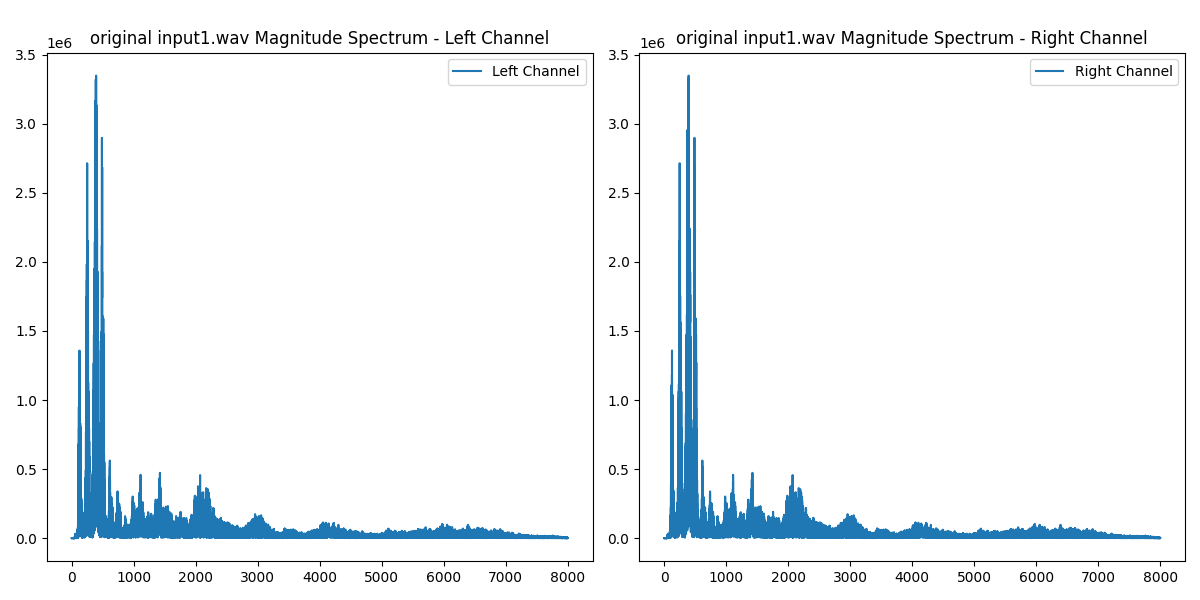
\includegraphics[width=\textwidth]{../data/input/magnitude_spectrum/original_input1.wav_magnitude_spectrum.png}
        \caption{Magnitude Spectrum Before Filtering}
    \end{minipage} \hfill
    \begin{minipage}{1\textwidth}
        \centering
        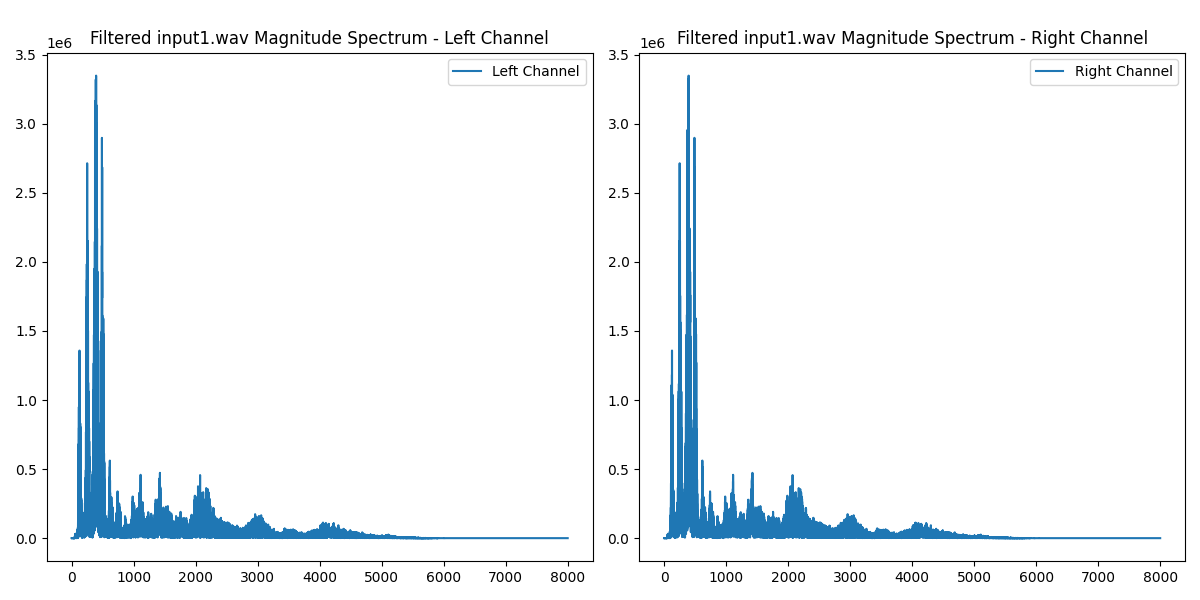
\includegraphics[width=\textwidth]{../data/filtered/magnitude_spectrum/filtered_input1.wav_magnitude_spectrum.png}
        \caption{Magnitude Spectrum After Filtering}
    \end{minipage}
\end{figure}

\newpage

\section{SSB Modulation}

\subsection{Carrier Frequency Selection}
Carrier frequencies were chosen as \texttt{6K}, \texttt{11K}, and \texttt{16K} Hz. These frequencies ensure that the modulated signals do not overlap in the frequency domain, which is critical for avoiding interference during demodulation.
Due to not using an ideal filter, a gap of 5 kHz between the carrier frequencies, which exceeds the filter’s cutoff frequency of 4 kHz, provides sufficient separation between the signals.

\subsection{Implementation of SSB Modulation}

In this section, we outline the implementation of Single Sideband (SSB) Modulation. The process involves two key steps: Double Sideband (DSB) Modulation and filtering to isolate the desired sideband. Below, we detail each step with placeholders for code snippets and graphical representations of the results.

\subsubsection{Step 1: Double Sideband (DSB) Modulation}
To perform DSB Modulation, the input signal is multiplied with a carrier signal. Different carrier frequencies are chosen for each signal to ensure proper modulation. This can be expressed mathematically as:
\[ s_{DSB}(t) = m(t) \cdot \cos(2\pi f_c t), \]
where \( m(t) \) is the input signal and \( f_c \) is the carrier frequency. \\
\\
Below is the code used for DSB Modulation:
\begin{lstlisting}[language=Python, caption=DSB Modulation Code]
# Apply DSB modulation to the left channel of the signal
sample_rate, signal = read(os.path.join(filtered_dir, file))
left_channel = signal[:, 0]
t = np.linspace(0, DURATION, sample_rate * DURATION, endpoint=False)
carrier = np.cos(2 * np.pi * carrier_frequencies[i] * t)
modulated_left = left_channel * carrier
\end{lstlisting}
Below is the graphical representation of the DSB-modulated signals for each input signal:

\begin{figure}[H]
    \centering
    \begin{minipage}{0.29\textwidth}
        \centering
        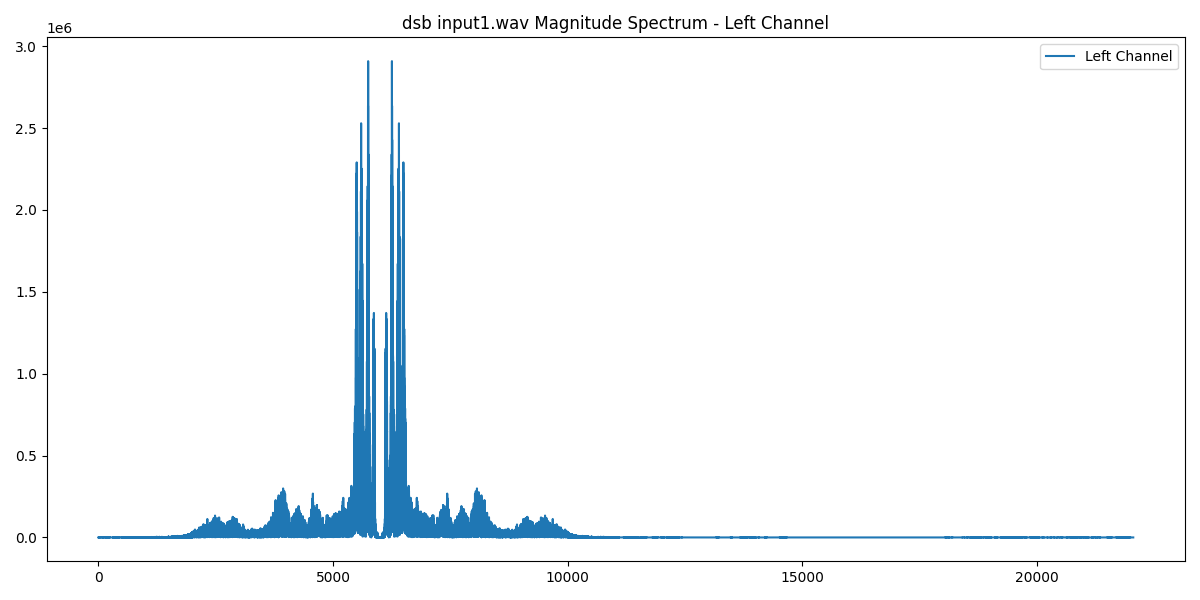
\includegraphics[width=\textwidth]{../data/modulated/dsb_spectrum/dsb_input1.wav_magnitude_spectrum.png}
    \end{minipage} \hfill
    \begin{minipage}{0.29\textwidth}
        \centering
        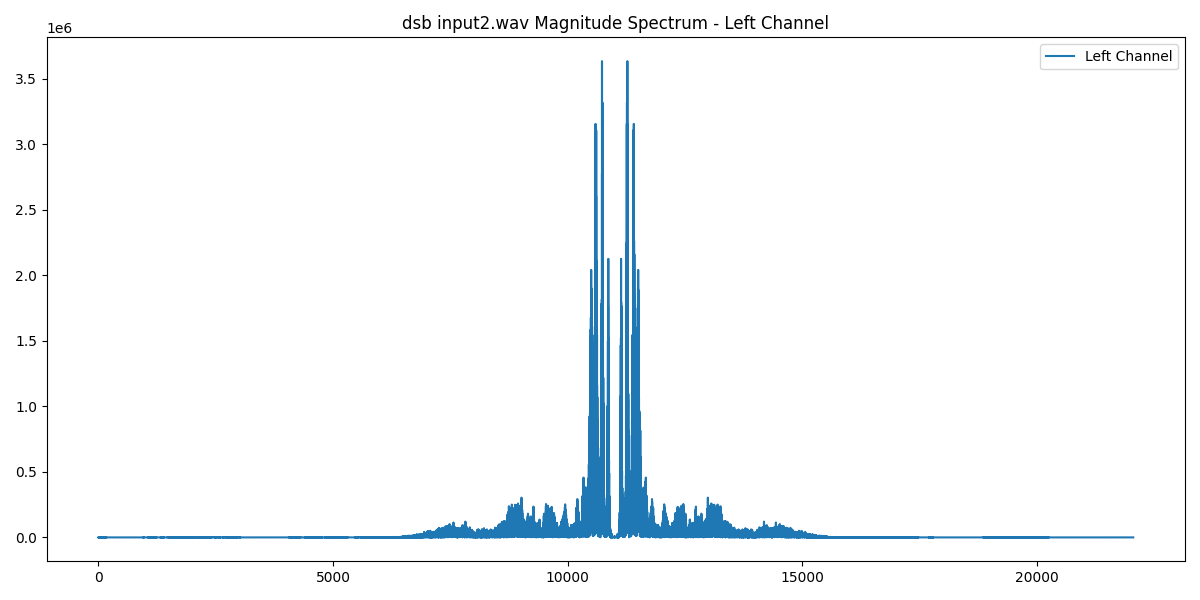
\includegraphics[width=\textwidth]{../data/modulated/dsb_spectrum/dsb_input2.wav_magnitude_spectrum.png}
    \end{minipage} \hfill
    \begin{minipage}{0.29\textwidth}
        \centering
        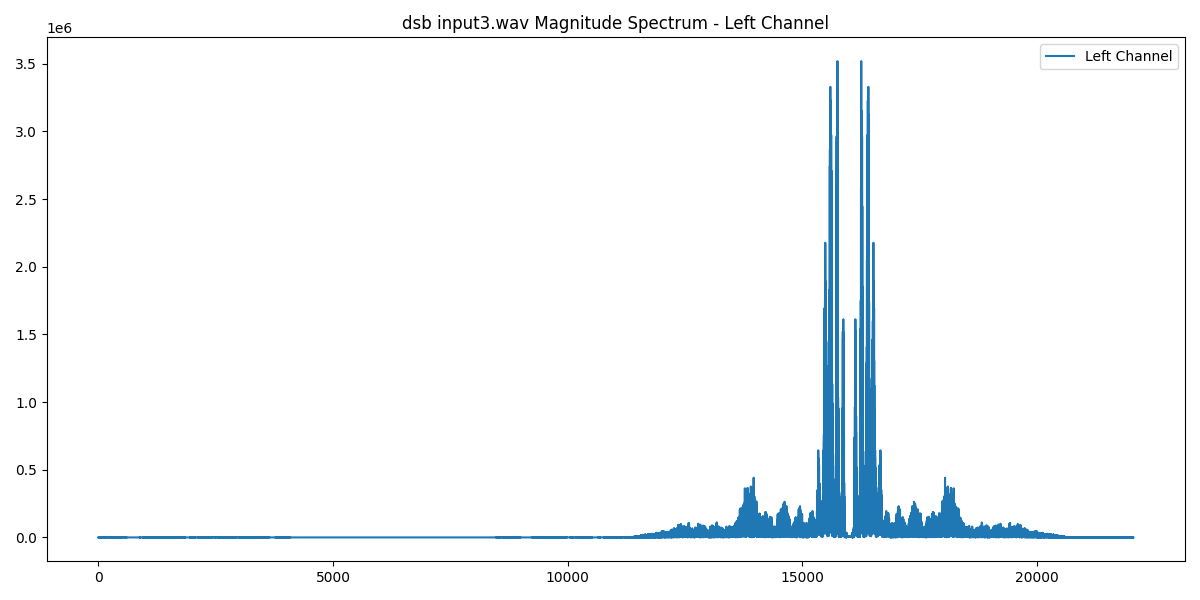
\includegraphics[width=\textwidth]{../data/modulated/dsb_spectrum/dsb_input3.wav_magnitude_spectrum.png}
    \end{minipage}
    \caption{Magnitude Spectrum of DSB-Modulated Signals}
\end{figure}


\subsubsection{Step 2: High-Pass Filtering to Obtain the Upper Sideband}
After DSB Modulation, a high-pass filter is applied to extract the upper sideband (USB) of the signal. The filtering operation removes the lower sideband (LSB), leaving only the USB component. The high-pass filter is designed with a cutoff frequency just above the carrier frequency. \\
\\
Below is the code used for high-pass filtering to isolate the upper sideband:
\begin{lstlisting}[language=Python, caption=High-Pass Filtering Code]
# Normalize the carrier frequency to the Nyquist frequency (half the sample rate)
nyquist_freq = sample_rate / 2.0
normalized_cutoff = carrier_freq / nyquist_freq

# Design a Butterworth high-pass filter
sos = butter(order, normalized_cutoff, btype='high', analog=False, output='sos')

# Apply the filter to the signal
filtered_signal = sosfilt(sos, signal)
\end{lstlisting}
The magnitude spectrum of the SSB-modulated signals is shown below:

\begin{figure}[H]
    \centering
    \begin{minipage}{0.29\textwidth}
        \centering
        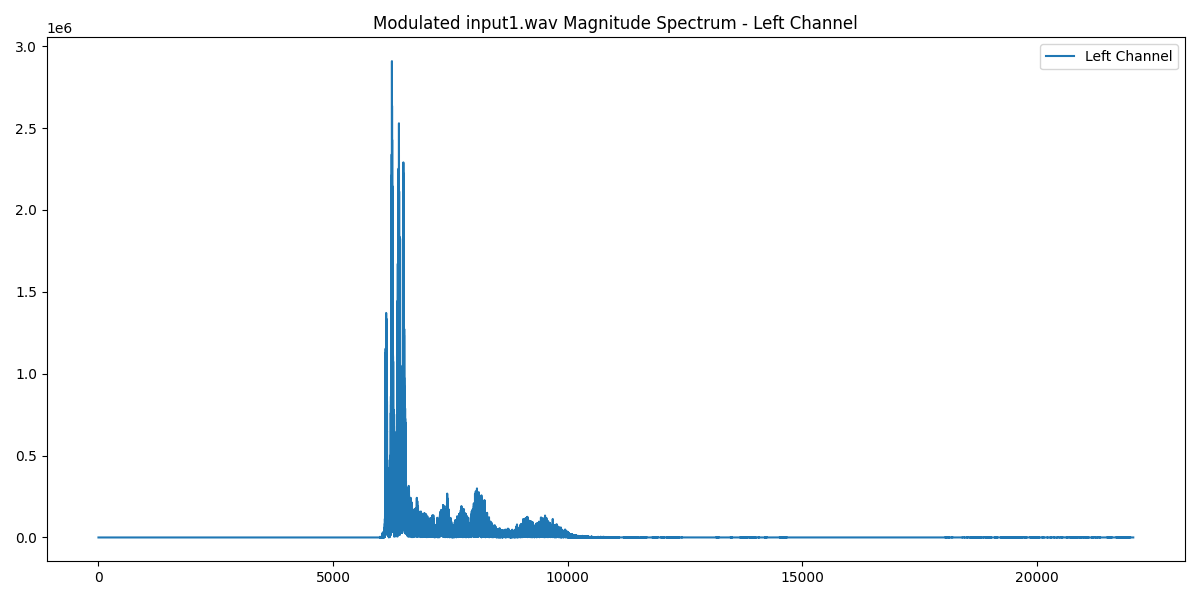
\includegraphics[width=\textwidth]{../data/modulated/magnitude_spectrum/modulated_input1.wav_magnitude_spectrum.png}
    \end{minipage} \hfill
    \begin{minipage}{0.29\textwidth}
        \centering
        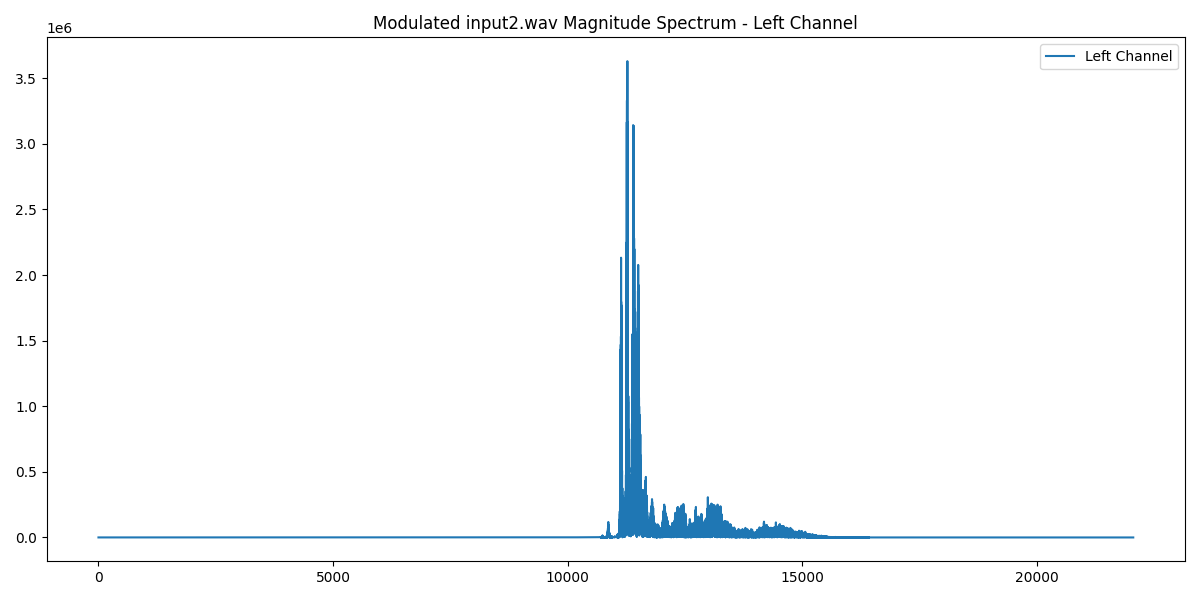
\includegraphics[width=\textwidth]{../data/modulated/magnitude_spectrum/modulated_input2.wav_magnitude_spectrum.png}
    \end{minipage} \hfill
    \begin{minipage}{0.29\textwidth}
        \centering
        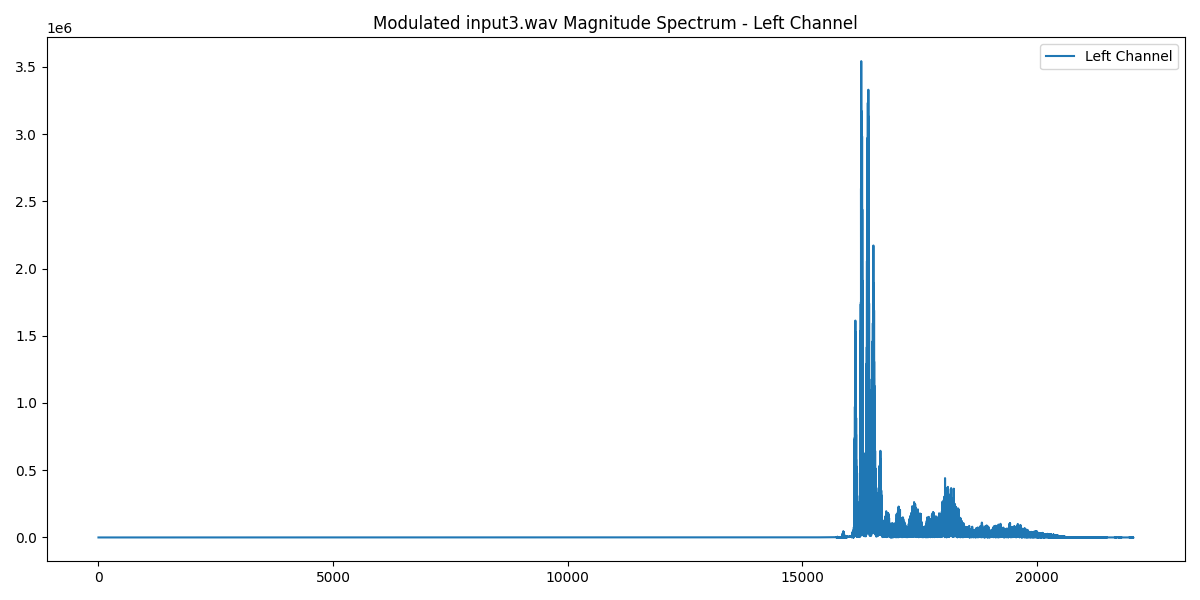
\includegraphics[width=\textwidth]{../data/modulated/magnitude_spectrum/modulated_input3.wav_magnitude_spectrum.png}
    \end{minipage}
    \caption{Magnitude Spectrum of SSB-Modulated Signals}
\end{figure}

\newpage

\section{Frequency Division Multiplexing (FDM)}

\subsection{Multiplexing Process}
The multiplexing process involves combining the SSB-modulated signals into a single composite signal. \\
\\
Below is the code used for FDM Multiplexing:
\begin{lstlisting}[language=Python, caption=FDM Multiplexing Code]
# Combine the modulated signals
modulated_signals = [modulated_input1, modulated_input2, modulated_input3]
fdm_signal = np.sum(modulated_signals, axis=0)
\end{lstlisting}
The magnitude spectrum of the multiplexed signal is shown below:
\begin{figure}[H]
    \centering
    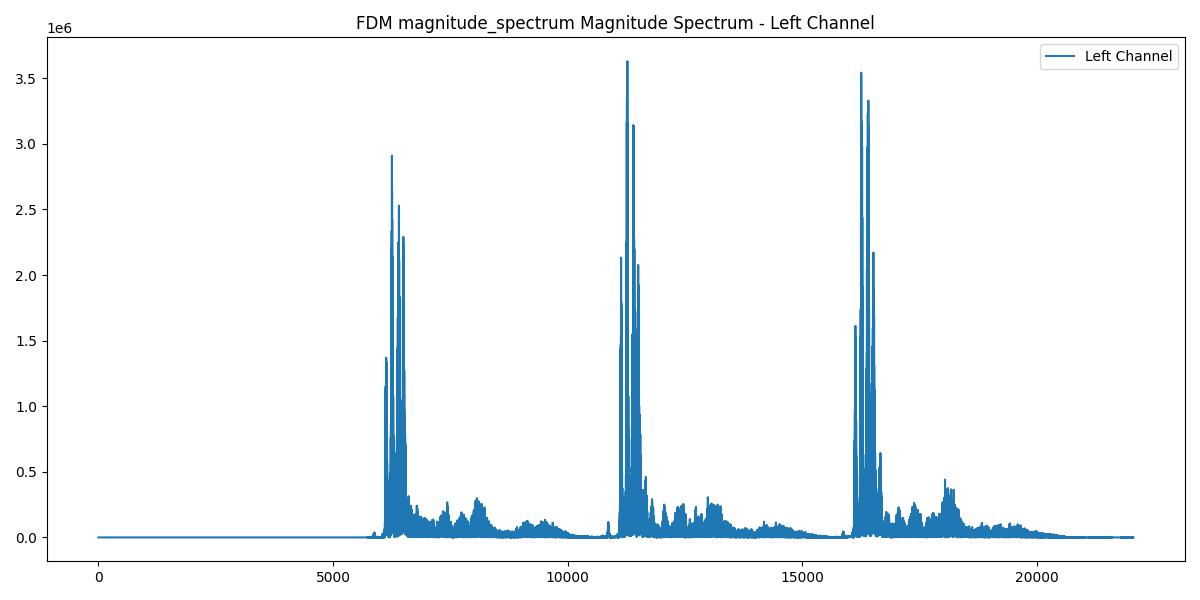
\includegraphics[width=0.8\textwidth]{../data/modulated/fdm_spectrum/FDM_magnitude_spectrum_magnitude_spectrum.png}
    \caption{Magnitude Spectrum of Multiplexed Signals}
\end{figure}

\newpage

\section{SSB Demodulation and Signal Recovery}

In this section, we describe the implementation of Single Sideband (SSB) demodulation and signal recovery. The process involves applying a bandpass filter to isolate each signal, followed by demodulation using multiplication with a cosine wave. Finally, the signal is scaled to its original amplitude.

\subsubsection{Step 1: Bandpass Filtering to Isolate Each Signal}
To recover individual signals, a bandpass filter is applied to extract each frequency band corresponding to the desired signal. The bandpass filter is designed with a passband centered around the carrier frequency for each signal. This ensures that only the desired signal is retained for further processing. Mathematically, this step isolates:
\[ s_{BPF}(t) = H_{BP}(f) \cdot s_{SSB}(t), \]
where \( H_{BP}(f) \) is the transfer function of the bandpass filter. \\
\\
Below is the code used for bandpass filtering:
\begin{lstlisting}[language=Python, caption=Bandpass Filtering Code]
# Apply bandpass filtering to isolate each signal
nyquist_freq = sample_rate / 2.0
low = low_cutoff / nyquist_freq
high = high_cutoff / nyquist_freq
sos = butter(order, [low, high], btype='band', analog=False, output='sos')
filtered_signal = sosfilt(sos, signal)
\end{lstlisting}

The magnitude spectrum of the bandpass-filtered signals is shown below:
\begin{figure}[H]
    \centering
    \begin{minipage}{0.29\textwidth}
        \centering
        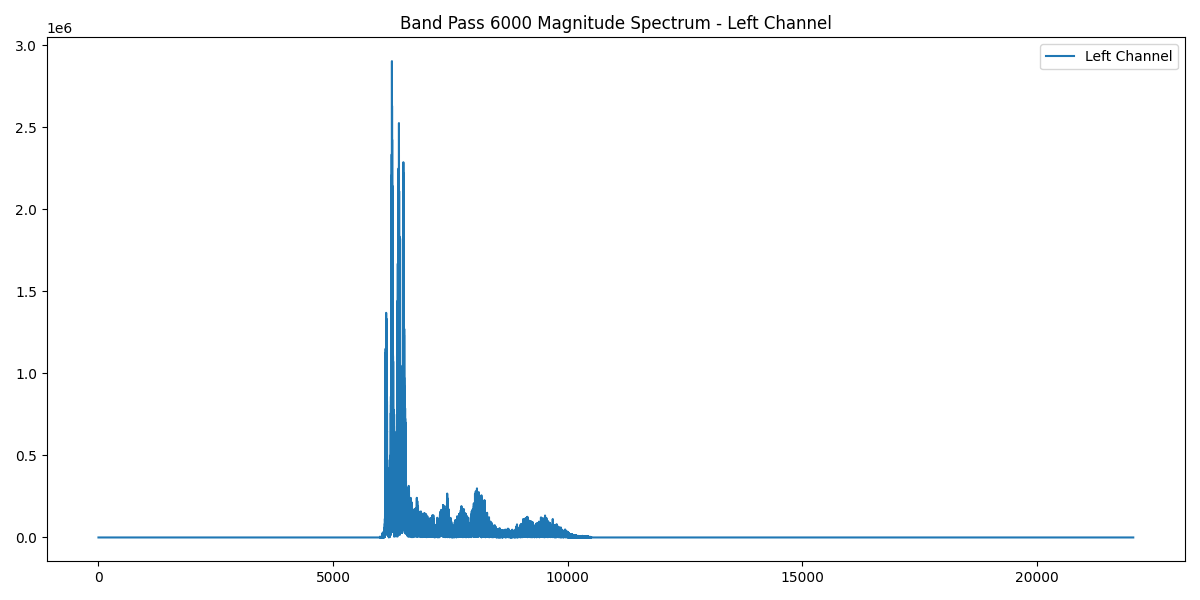
\includegraphics[width=\textwidth]{../data/demodulated/separated_spectrums/band_pass_6000_magnitude_spectrum.png}
    \end{minipage} \hfill
    \begin{minipage}{0.29\textwidth}
        \centering
        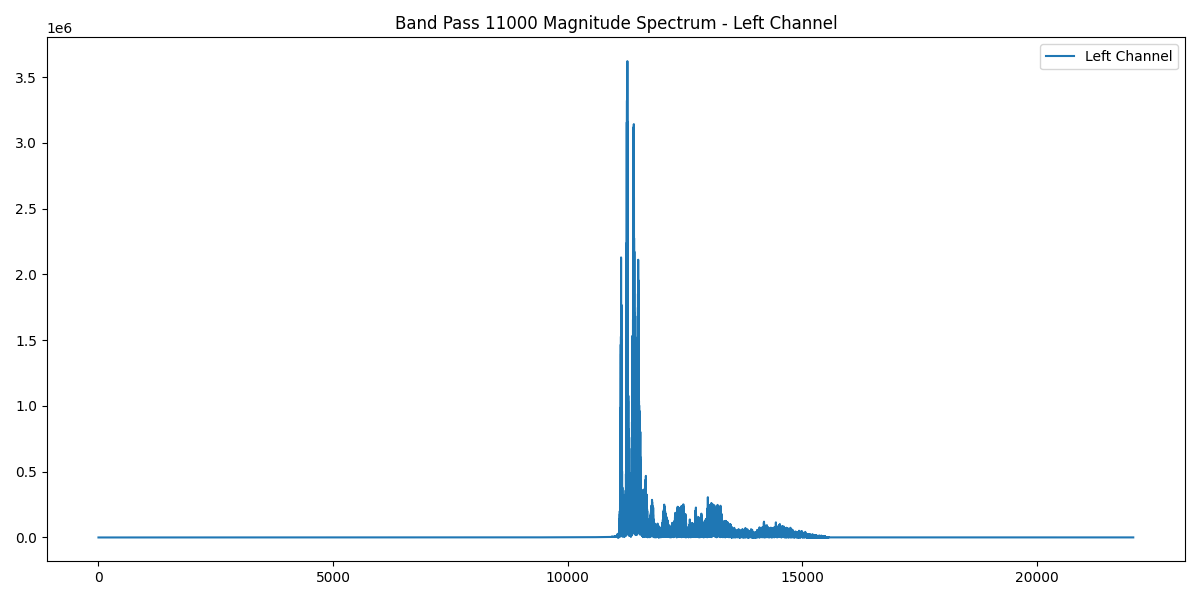
\includegraphics[width=\textwidth]{../data/demodulated/separated_spectrums/band_pass_11000_magnitude_spectrum.png}
    \end{minipage} \hfill
    \begin{minipage}{0.29\textwidth}
        \centering
        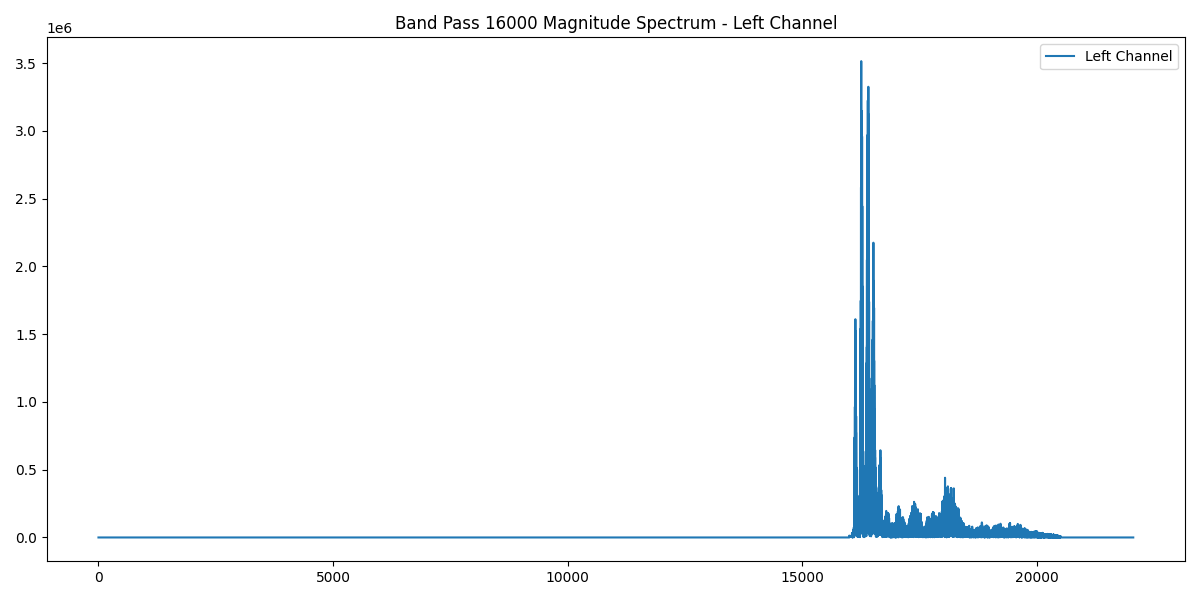
\includegraphics[width=\textwidth]{../data/demodulated/separated_spectrums/band_pass_16000_magnitude_spectrum.png}
    \end{minipage}
    \caption{Magnitude Spectrum of Bandpass Filtered Signals}
\end{figure}

\subsubsection{Step 2: Demodulation to Recover the Original Signal}
After isolating the desired signal, it is multiplied with a cosine wave of the corresponding carrier frequency to demodulate it back to its baseband form. This operation effectively reverses the modulation process:
\[ s_{demod}(t) = s_{BPF}(t) \cdot \cos(2\pi f_c t). \]

To restore the signal's amplitude, we multiply it by a factor of 4, as both modulation and demodulation reduce the amplitude by half each. \\
\\
Below is the code used for demodulation:
\begin{lstlisting}[language=Python, caption=Demodulation Code]
# Demodulate the signal using a cosine wave
sample_rate, signal = read(os.path.join(separated_audios_dir, file))
t = np.linspace(0, DURATION, sample_rate * DURATION, endpoint=False)  # Time vector
carrier = np.cos(2 * np.pi * carrier_frequencies[i] * t)
demodulated_signal = AMPLIFING_FACTOR * signal * carrier
demodulated_signal = Filterer.low_pass_filter(demodulated_signal, sample_rate, LIMIT_FREQUENCY, FilterType.LOW_PASS_BUTTERWORTH)
\end{lstlisting}

The demodulated signals for each input signal are shown below:
\begin{figure}[H]
    \centering
    \begin{minipage}{0.29\textwidth}
        \centering
        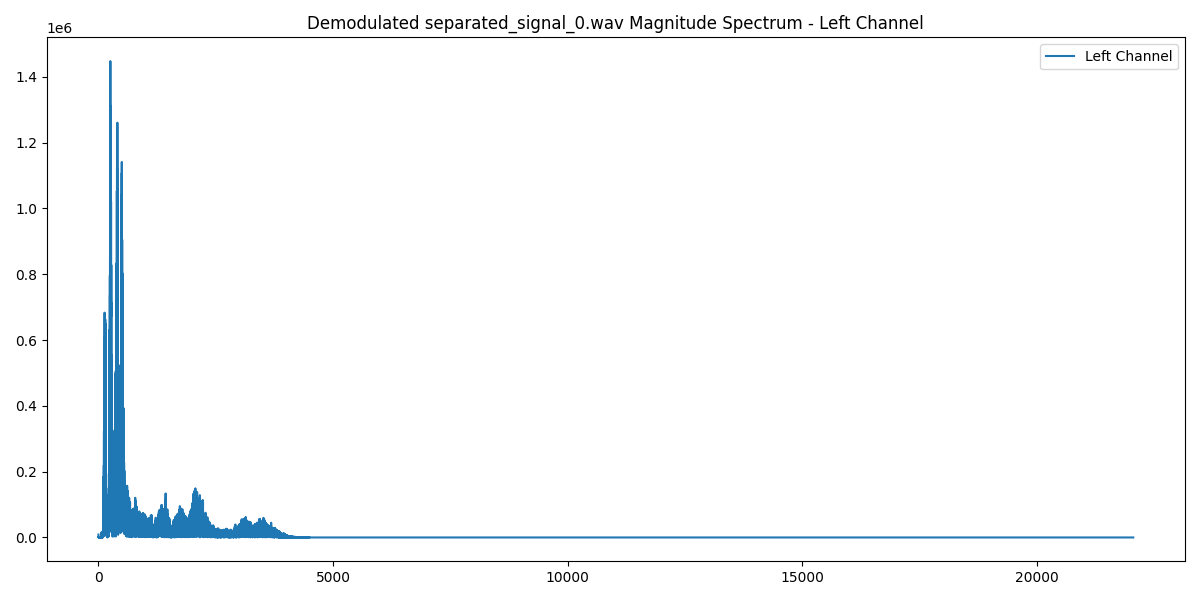
\includegraphics[width=\textwidth]{../data/demodulated/signals_after_demodulation_spectrum/out0.png}
    \end{minipage} \hfill
    \begin{minipage}{0.29\textwidth}
        \centering
        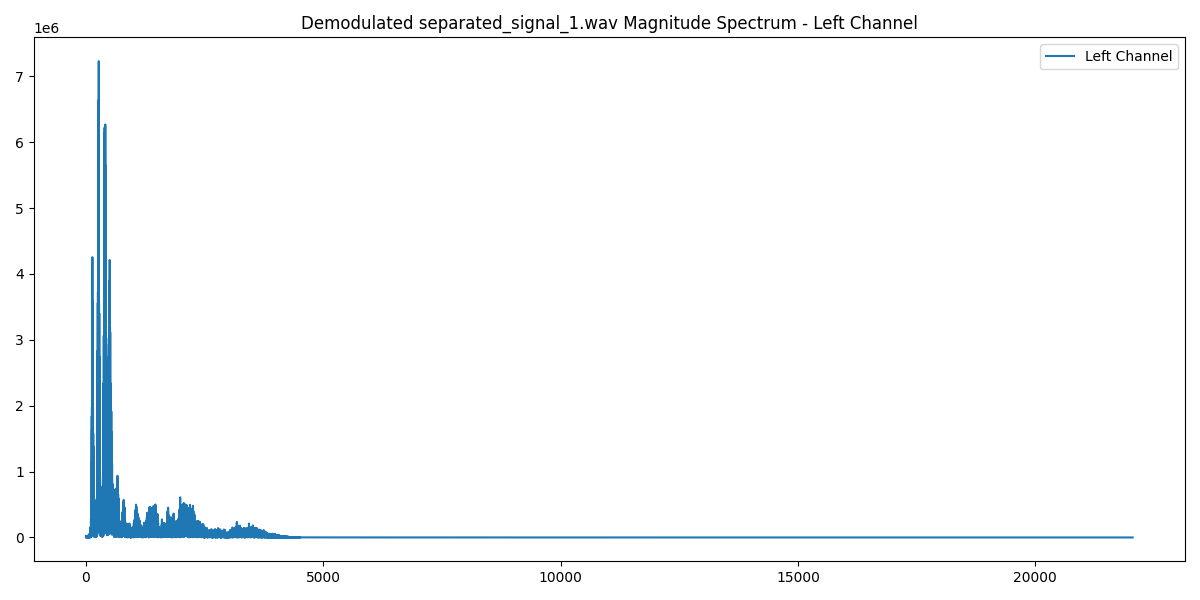
\includegraphics[width=\textwidth]{../data/demodulated/signals_after_demodulation_spectrum/out1.png}
    \end{minipage} \hfill
    \begin{minipage}{0.29\textwidth}
        \centering
        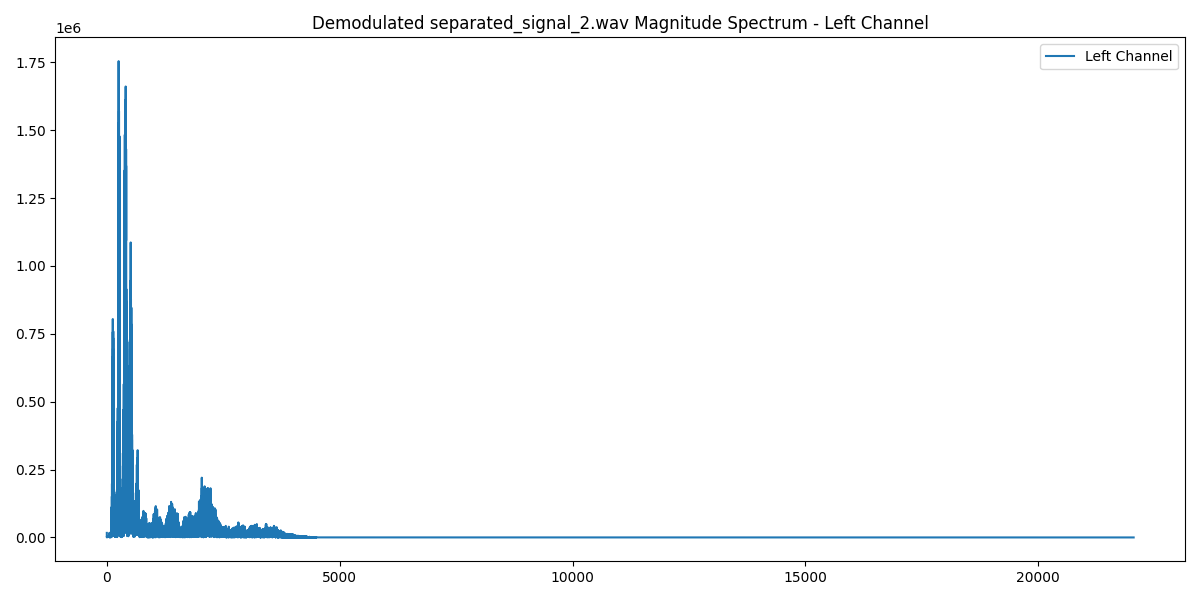
\includegraphics[width=\textwidth]{../data/demodulated/signals_after_demodulation_spectrum/out2.png}
    \end{minipage}
    \caption{Magnitude Spectrum of Bandpass Filtered Signals}
\end{figure}


By following the above steps, we successfully recover the original signal from its SSB-modulated form, restoring it to its initial amplitude and frequency domain characteristics.

Summarize the outcomes of the project, key findings, and possible improvements for future work.

\newpage
\section*{Appendix: Code}
Below is the full Python code used in the project:
% Add commmon_includes.py file
\lstinputlisting[language=Python, caption=Common Includes]{../src/common_includes.py}
% Add record_audio.py file
\lstinputlisting[language=Python, caption=Record Audio]{../src/record_audio.py}
% Add filterer.py file
\lstinputlisting[language=Python, caption=Filterer]{../src/filter_signal.py}
% Add modulator.py file
\lstinputlisting[language=Python, caption=Modulator]{../src/modulator.py}
% Add demodulator.py file
\lstinputlisting[language=Python, caption=Demodulator]{../src/demodulator.py}
% Add plot_signal.py file
\lstinputlisting[language=Python, caption=Plot Signal]{../src/plot_signal.py}
\newpage

\end{document}
